%!TEX TS-program = xelatex
%  Lab0.Rnw
%
%  Created by David Rosenberg on 2009-09-10.
%  Copyright (c) 2009 University of Chicago. All rights reserved.
%
\documentclass[10pt,letterpaper]{article}
\usepackage[Rpdflatex]{Rosenberg}
\usepackage{svn-multi}
\usepackage{tikz}

\svnidlong
{$LastChangedDate: 2009-10-05 15:42:55 -0500 (Mon, 05 Oct 2009) $}
{$LastChangedRevision: 80 $}
{$LastChangedBy: root $}
% \svnid{$Id: example_main.tex 146 2008-12-03 13:29:19Z martin $}
% Don't forget to set the svn property 'svn:keywords' to
% 'HeadURL LastChangedDate LastChangedRevision LastChangedBy' or
% 'Id' or both depending if you use \svnidlong and/or \svnid
%
\newcommand{\svnfooter}{Last Changed Rev: \svnkw{LastChangedRevision}}
\svnRegisterAuthor{davidrosenberg}{David M. Rosenberg}


%\usepackage{Sweave}





\title{Introduction to computational programming\\\smaller Introductory Exercise\\\smaller Loops and flow control in \R}
\author{David M. Rosenberg\\\small University of Chicago\\\small Committee on Neurobiology\medskip\\
{\footnotesize \parbox[t]{10cm} {
Version control information:
\begin{tabbing}
\footnotesize\sffamily
 Last changes revision: \= \kill
 Last changed date: \> \svndate\\
 Last changes revision: \> \svnrev\\
 Version: \> \svnFullRevision*{\svnrev}\\
 Last changed by: \> David M. Rosenberg\\
\end{tabbing} 
}
}}

\begin{document}

\maketitle

\section*{Overview}

In this exercise we will explore the concepts of \emph{flow control} and \emph{loops}, two important tools for allowing the computer to do the ``work.''  We will start by reviewing \Rs facilities for boolean logic and how they enable simple control structures.  Next we will explore the use of loops to minimize repetitive chunks of code and the conventions for their use.

Don't forget to complete and submit the exercises at the end of this document to your TA.

\part{Tutorial}

\section{Flow control}

\subsection{Boolean Logic} % (fold)
\label{sub:boolean_logic}

One of the fundamental concepts of computer programming, and one often unfamiliar to non-programmers, is the concept of \emph{boolean logic}.  Boolean algebra is a simple mathematical system containing two values (\textbf{True} and \textbf{False}) and three operations (\textbf{AND}, \textbf{OR} and \textbf{NOT}).  The following table outlines how boolean logic is represented in \R.

\begin{center}
  \begin{tabular}{r l l l}
    \toprule
    & \R representation & context & meaning \\
    \midrule
    true & \texttt{TRUE} & \texttt{a} & \texttt{a} is true \\
    false & \texttt{FALSE} & \texttt{b} & \texttt{b} is true \\
    not & \texttt{!} & \texttt{!a} & inverse of \texttt{a} \\
    and & \texttt{\&} and \texttt{\&\&}\footnotemark[1] & \texttt{a \& b} & \texttt{a} and \texttt{b}\\
    or & \texttt{|} and \texttt{||}\footnotemark[1] & \texttt{a | b} & \texttt{a} or \texttt{b}\\
    \bottomrule
  \end{tabular}
\end{center}

\footnotetext[1]{The conjunction (\emph{and}) and disjunction (\emph{or}) each have two syntactical forms.  The single (\cc{\&} and \cc{|}) each return a logical \cc{vector} equal in length to the the length of their arguments (pairwise comparisons performed).  In contrast, the doubled forms (\cc{\&\&} and \cc{||}) return a single logical value which is \emph{TRUE} if and only if all pairwise comparisons are \emph{TRUE}.}


The conventions for using these operations are bit unusual.
\begin{itemize}
  \item \textbf{AND} (\texttt{\&}) takes two arguments, \texttt{a} and \texttt{b}.  One is placed before the \texttt{\&} and one after.  The expression \texttt{a \& b} evaluates to \texttt{TRUE} if and only if \texttt{a} evaluates to \texttt{TRUE} and \texttt{b} evaluates to \texttt{TRUE}.
  \item \textbf{OR} (\texttt{|}) takes two arguments, \texttt{a} and \texttt{b}.  One is placed before the \texttt{|} and one after.  The expression \texttt{a | b} evaluates to \texttt{TRUE} if \texttt{a} evaluates to \texttt{TRUE}, if \texttt{b} evaluates to \texttt{TRUE}, or if both \texttt{a} and \texttt{b} evaluate to \texttt{TRUE}.
  \item \textbf{NOT} (\texttt{!}) takes one argument, \texttt{a}, placed directly after the \texttt{!}.  The expression \texttt{!a} evaluates to \texttt{TRUE} if and only if \texttt{a} evaluates to \texttt{FALSE}.
\end{itemize}

Boolean logic is extremely important for \emph{conditionals}, which we will explore below.

One final aspect of \emph{boolean logic} which we must consider is that of \emph{boolean indexing}.  Recall that we can extract a subset of a vector by putting a vector of integer indexes in brackets.

\begin{Schunk}
\begin{Sinput}
> myVec <- letters
> myVec
\end{Sinput}
\begin{Soutput}
 [1] "a" "b" "c" "d" "e" "f" "g" "h" "i" "j" "k" "l" "m" "n" "o" "p" "q" "r" "s"
[20] "t" "u" "v" "w" "x" "y" "z"
\end{Soutput}
\begin{Sinput}
> myVec[1:5]          # First five letters
\end{Sinput}
\begin{Soutput}
[1] "a" "b" "c" "d" "e"
\end{Soutput}
\end{Schunk}

You can also use a \emph{logical vector} (a vector of only \texttt{TRUE} or \texttt{FALSE} members) to index a vector as well.  The result of such an operation is a vector composed of all the members of the original vector which were indexed by \texttt{TRUE}.  An example may help to clarify this

\begin{Schunk}
\begin{Sinput}
> myVec <- letters
> myVec
\end{Sinput}
\begin{Soutput}
 [1] "a" "b" "c" "d" "e" "f" "g" "h" "i" "j" "k" "l" "m" "n" "o" "p" "q" "r" "s"
[20] "t" "u" "v" "w" "x" "y" "z"
\end{Soutput}
\begin{Sinput}
> idx <- 1:26
> bool_idx <- idx < 10              # logical vector
> bool_idx
\end{Sinput}
\begin{Soutput}
 [1]  TRUE  TRUE  TRUE  TRUE  TRUE  TRUE  TRUE  TRUE  TRUE FALSE FALSE FALSE
[13] FALSE FALSE FALSE FALSE FALSE FALSE FALSE FALSE FALSE FALSE FALSE FALSE
[25] FALSE FALSE
\end{Soutput}
\begin{Sinput}
> myVec[bool_idx]                   # the first 10 letters of the alphabet
\end{Sinput}
\begin{Soutput}
[1] "a" "b" "c" "d" "e" "f" "g" "h" "i"
\end{Soutput}
\end{Schunk}

% subsection boolean_logic (end)

\subsubsection{Conditionals} % (fold)
\label{ssub:conditionals}

Conditionals are ``tests'' which return either \texttt{TRUE} or \texttt{FALSE} with respect to a particular variable.  The most familiar conditionals are likely the \emph{comparison operators}

\bc
  \begin{tabular}{r c c l }
  \toprule
  comparison & \R representation & context & notes \\
  \midrule
  equality & \texttt{==} & \texttt{a == b} & True if \texttt{a} and \texttt{b} have the same value \\
  inequality & \texttt{!=} & \texttt{a != b} & synonomous with \texttt{!(a == b)} \\
  less than, greater than & \texttt{<}, \texttt{>} & \texttt{a < b} & true if \texttt{a} is less than \texttt{b} \\
  less than or equal to & \texttt{<=}, \texttt{>=} & \texttt{a <= b} & synonomous with \texttt{(a < b) | (a == b)} \\
  set-theoretic inclusion & \texttt{\%in\%} & \texttt{a \%in\% b} & true if vector \texttt{b} contains \texttt{a} as one of its members \\
  vector union & \texttt{all()} & \texttt{all(a)} & true if every member of vector \texttt{a} is true \\
  vector intersection & \texttt{any()} & \texttt{any(a)} & true if any member of vector \texttt{a} is true \\
  \bottomrule
  \end{tabular}
\ec

The most basic use of conditionals involves the \R \texttt{if} command, which has the following syntax:

\begin{Schunk}
\begin{Sinput}
> if (CONDITION) {
+   BLOCK_1
+ } else if (CONDITION_2) {
+   BLOCK_2
+ } else {
+   ELSE_BLOCK
+ }
\end{Sinput}
\end{Schunk}
The capitalized expressions represent code which may be changed:
\bc
\begin{tabular}{r l}
  \toprule
expression & meaning \\
\midrule
\texttt{CONDITION} & a condition which evaluates to \texttt{TRUE} or \texttt{FALSE} \\
\texttt{BLOCK\_1} & a sequence of commands evaluated if \texttt{CONDITION} \\
                  &  evaluates to \texttt{TRUE} \\
\texttt{CONDITION\_2} (optional) & a second condition which is evaluated only if \texttt{CONDITION} \\
                  & evaluates to \texttt{FALSE}.  Note that as many \texttt{else if() } \\
                  & clauses may be used as one chooses. \\
\texttt{BLOCK\_2} (optional) & sequence of commands to be evaluated if \texttt{CONDITION\_2} \\
                  & is evaluated and \texttt{TRUE} \\
\texttt{ELSE\_BLOCK} (optional) & sequence of commands to be evaluated if none \\
                  & of the \texttt{CONDITION} blocks evaluate to be true.\\
\bottomrule
\end{tabular}
\ec

An example may help to clarify this syntax.

\begin{Schunk}
\begin{Sinput}
> x1 <- 2
> if (x1 < 10) {
+   cat(x1, " has only 1 digit.")
+ } else if (x1 < 100) {
+   cat(x1, " has two digits.")
+ } else if (x1 < 1000) {
+   cat(x1, " has three digits.")
+ } else {
+   cat(x1, " has more than three digits.")
+ }
> x1 <- 16
> if (x1 < 10) {
+   cat(x1, " has only 1 digit.")
+ } else if (x1 < 100) {
+   cat(x1, " has two digits.")
+ } else if (x1 < 1000) {
+   cat(x1, " has three digits.")
+ } else {
+   cat(x1, " has more than three digits.")
+ }
> x1 <- 128
> if (x1 < 10) {
+   cat(x1, " has only 1 digit.")
+ } else if (x1 < 100) {
+   cat(x1, " has two digits.")
+ } else if (x1 < 1000) {
+   cat(x1, " has three digits.")
+ } else {
+   cat(x1, " has more than three digits.")
+ }
> x1 <- 1024
> if (x1 < 10) {
+   cat(x1, " has only 1 digit.")
+ } else if (x1 < 100) {
+   cat(x1, " has two digits.")
+ } else if (x1 < 1000) {
+   cat(x1, " has three digits.")
+ } else {
+   cat(x1, " has more than three digits.")
+ }
\end{Sinput}
\end{Schunk}

This example should produce the following output:
\begin{Schunk}
\begin{Soutput}
2  has only 1 digit.
\end{Soutput}
\begin{Soutput}
16  has two digits.
\end{Soutput}
\begin{Soutput}
128  has three digits.
\end{Soutput}
\begin{Soutput}
1024  has more than three digits.
\end{Soutput}
\end{Schunk}
% subsubsection conditionals (end)


\subsubsection{Flow control / loops} % (fold)
\label{ssub:flow_control_loops}

\emph{Flow control}, the process by which commands are ``selected'' and evaluated is defined by two major constructs: \emph{conditionals} (seen in the previous section) and \emph{Loops}.  A \emph{loop} is a section of code which is repeatedly evaluated (often with variables assuming different values).  In \R, there are two main types of loops which we will consider.

\emph{While} loops are used to evaluate a set of commands based on the result of a \emph{conditional} test.  The syntax for a \texttt{while} loop is as follows:

\begin{Schunk}
\begin{Sinput}
> while(CONDITION) {
+   BLOCK
+ }
\end{Sinput}
\end{Schunk}
Here, \texttt{\emph{CONDITION}} is a conditional statement (see above), and \texttt{\emph{BLOCK}} is a series of commands which are evaluated, in sequence, until \texttt{\emph{CONDITION}} evaluates to \texttt{FALSE}.  As an example, consider the fibonacci sequence $f_n=0, 1, 1, 2, 3, 5, \ldots$, defined by:
\begin{equation}
  f_n = \begin{cases}
  0 & \text{ if  $n=1$, }\\
  1, & \text{ if  $n=2$, }\\
  f_{n-1} + f_{n-2}, & \text{ if  $n > 2$}\\
\end{cases}
\end{equation}
Suppose that we wanted to find the first number in the fibonacci sequence greater than 1000.

\begin{Schunk}
\begin{Sinput}
> x0 <- 0
> x1 <- 1
> while(x1 < 1000) {      # x1 < 1000 is the condition
+   newX1 <- x0 + x1      # -\
+   x0 <- x1              # --+ -- these three lines make up the BLOCK
+   x1 <- newX1           # -/
+ }
> x1
\end{Sinput}
\begin{Soutput}
[1] 1597
\end{Soutput}
\end{Schunk}

The second of our looping constructs, the \texttt{for} loop, is used to repeat a sequence of commands a predetermined number of times.

\begin{Schunk}
\begin{Sinput}
> for (COUNTER in VECTOR) {
+   BLOCK
+ }
\end{Sinput}
\end{Schunk}

Here \texttt{\emph{COUNTER}} is a variable which changes from one iteration of the loop to the next and \texttt{\emph{VECTOR}} is a vector of values.  \texttt{\emph{BLOCK}} is evaluated once for each value in \texttt{\emph{VECTOR}}.  In each iteration, \texttt{\emph{COUNTER}} is assigned a new value, taken from the members of \texttt{\emph{VECTOR}}.

Continuing with the previous example, suppose now you wanted to know the first 20 values of the fibonacci sequence.  Then:

\begin{Schunk}
\begin{Sinput}
> xVec <- c(0, 1)
> for (ii in 3:20){
+   xminus1 <- xVec[ii-1]
+   xminus2 <- xVec[ii-2]
+   newVal <- xminus1 + xminus2
+   xVec <- c(xVec, newVal)
+ }
> xVec
\end{Sinput}
\begin{Soutput}
 [1]    0    1    1    2    3    5    8   13   21   34   55   89  144  233  377
[16]  610  987 1597 2584 4181
\end{Soutput}
\end{Schunk}

There are two special commands for dealing with loops
\begin{itemize}
  \item \texttt{break} immediately terminates the loop and continues evaluation at the first command following the end brace of the loop. 
  \item \texttt{next} ends the current loop iteration and starts the next one.
\end{itemize}

% subsubsection flow_control_loops (end)

\section{Complex numbers} % (fold)
\label{sec:complex_numbers}


\subsection{Syntax} % (fold)
\label{sub:syntax}

As you (may) recall from the \textbf{Guide to Using \emph{R}}, the \R interpreter has built-in support for complex numbers.  Shown below are example code for generating complex values in \R and a summary of the five major complex operations supported by \emph{R}.

\begin{Schunk}
\begin{Sinput}
> myVar <- 3 + 4i
> myVar
\end{Sinput}
\begin{Soutput}
[1] 3+4i
\end{Soutput}
\begin{Sinput}
> is.complex(3 + 4i)
\end{Sinput}
\begin{Soutput}
[1] TRUE
\end{Soutput}
\begin{Sinput}
> is.complex(3)
\end{Sinput}
\begin{Soutput}
[1] FALSE
\end{Soutput}
\begin{Sinput}
> myVar2 <- complex(real=3, imaginary=4)
> myVar3 <- complex(argument=0.9272952, modulus=5)
> myVar2
\end{Sinput}
\begin{Soutput}
[1] 3+4i
\end{Soutput}
\begin{Sinput}
> myVar3
\end{Sinput}
\begin{Soutput}
[1] 3+4i
\end{Soutput}
\end{Schunk}

\bc
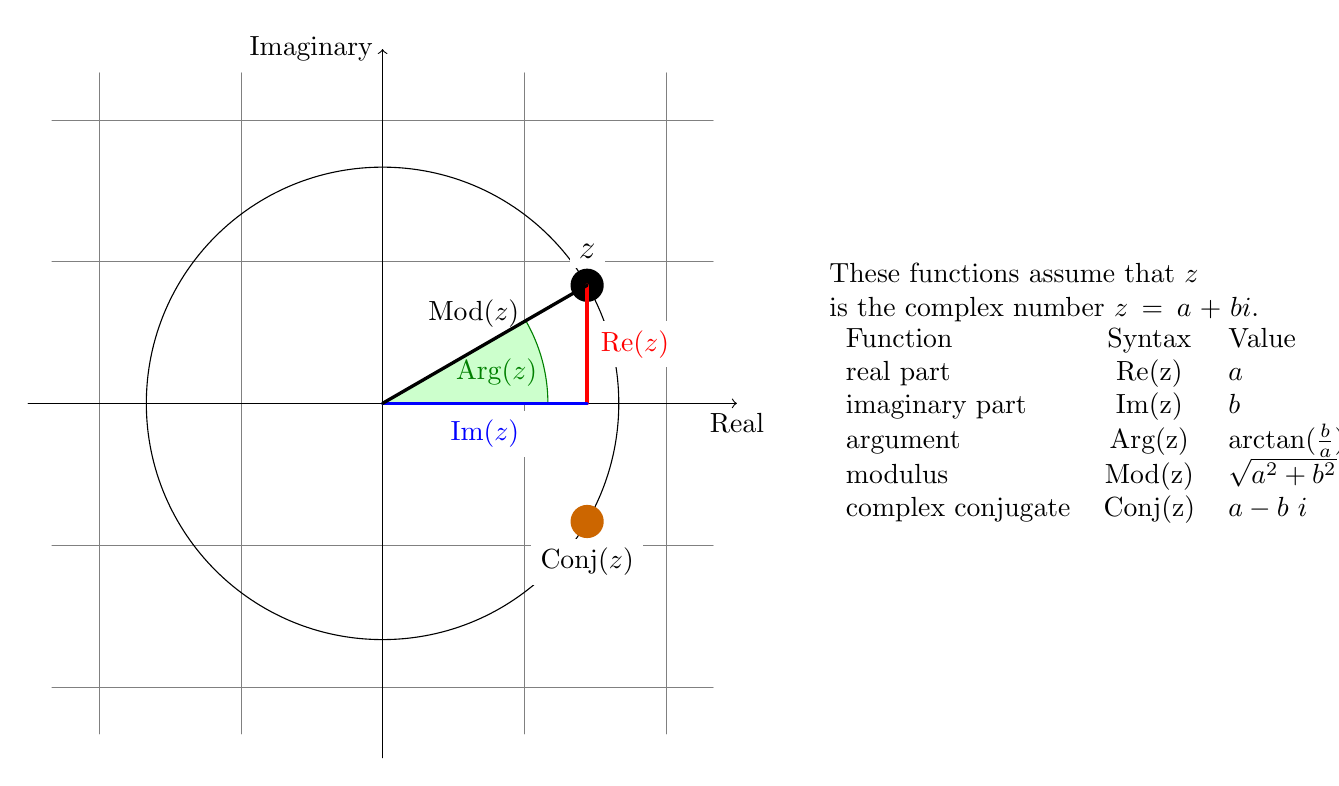
\begin{tikzpicture}[scale=3,cap=round]
  % Local definitions
  \def\costhirty{0.8660256}
  \def\sinthirty{0.5}
  % Colors
  \colorlet{anglecolor}{green!50!black}
  \colorlet{sincolor}{red}
  \colorlet{tancolor}{orange!80!black}
  \colorlet{coscolor}{blue}

  % Styles
  \tikzstyle{axes}=[]
  \tikzstyle{important line}=[very thick]
  %\tikzstyle{information text}=[rounded corners,fill=red!10,inner sep=1ex]

  % The graphic
  \draw[style=help lines,step=0.6cm] (-1.4,-1.4) grid (1.4,1.4);

  \draw (0,0) circle (1cm);

  \begin{scope}[style=axes]
    \draw[->] (-1.5,0) -- (1.5,0) node[below] {Real};
    \draw[->] (0,-1.5) -- (0,1.5) node[left] {Imaginary};
  \end{scope}
  % The graphic
  \filldraw[fill=green!20,draw=anglecolor] (0,0) -- (7mm,0pt) arc(0:30:7mm);


  \fill [tancolor,opacity=1.0] (\costhirty, -0.5) circle (2pt);
  \fill [black,opacity=1.0] (\costhirty, 0.5) circle (2pt);

  \draw (\costhirty, 0.5) node[above=6pt,fill=white] {\large $z$};
  \draw (\costhirty, -0.5) node[below=6pt,fill=white] {\cc{Conj}($z$)};

  \draw (15:5mm) node[anglecolor] {\cc{Arg}($z$)};

  \draw[style=important line,sincolor]
    (30:1cm) -- node[right=1pt,fill=white] {\cc{Re}($z$)} +(0,-.5);

  \draw[style=important line,coscolor]
    (0,0) -- node[below=2pt,fill=white] {\cc{Im}($z$)} (\costhirty,0);

  \draw [style=important line,black] (0, 0) -- node[left=4pt,above=2pt] {\cc{Mod}($z$)} (\costhirty, 0.5);

  \draw[xshift=1.85cm] node [right,text width=6cm]
    {
    \centering
    These functions assume that $z$ is the complex number $z=a + b i$.
    \medskip
    \begin{tabular}{l c l}
      \toprule
      Function & Syntax & Value\\
      \midrule
      real part & \cc{Re(z)} & $a$ \\
      imaginary part & \cc{Im(z)} & $b$ \\
      argument & \cc{Arg(z)} & $\arctan (\frac{b}{a})$ \\
      modulus & \cc{Mod(z)} & $\sqrt{a^2 + b^2}$ \\
      complex conjugate & \cc{Conj(z)} & $a - b\ i$ \\
      \bottomrule
    \end{tabular}
    };
\end{tikzpicture}
\ec


% subsection special_functions (end)

% section complex_numbers (end)



\part{Exercises} % (fold)
\label{prt:exercises}

\begin{enumerate}
  \item \begin{enumerate}
    \item  Starting with the fibonacci sequence examples from the tutorial, write a code chunk which takes as input a number \Com{k} and finds the largest fibonacci number less than or equal to \Com{k}
    \item Write a code chunk which takes as input three numbers (say, \Com{k}, \Com{x}, and \Com{y}) and prints either the second number (\Com{x}) or the third number (\Com{y}) depending on which is closer to \Com{k}.  (\emph{Hint:} the functions \Com{min()}, \Com{max()}, and \Com{abs()} may be helpful.  See the online documentation for their usage.)
    \item Write a code chunk which takes as input a number \Com{k} and returns the fibonacci number with is closest to \Com{k}.
  \end{enumerate}
  \item \begin{enumerate}
    \item Write a code chunk which takes a ``sorted'' numeric vector of length 2 and another numeric vector of length 1 and prints a single ``sorted'' vector of length 3.
    \item Write a code chunk which takes an ``unsorted'' numeric vector of length 2 and prints the values of that vector, ``sorted.''
    \item Write a code chunk that takes an ``unsorted'' numeric vector of length 10 and prints the sorted values to the screen.
  \end{enumerate}
  \item Consider the equation
  \begin{equation}
    x ^ k - 1 = 0, \quad x \in \mathbb{C}, \, k \in \mathbb{N}
  \end{equation}
  Write a code chunk that takes in integer ($k$) as input and prints all values $x$ which satisfy the above equation.
\end{enumerate}

\end{document}

